\subsection{Approach}
\label{sec:hard_cut_approach}

Hard cuts are abrupt transitions from one scene to another. 
Normally the content of the two frames involved in such a cut is highly different, see Figure~\ref{fig:hard_cut_example}, while two consecutive frames in one scene will not differ that much. 

\begin{figure}
	\centering
	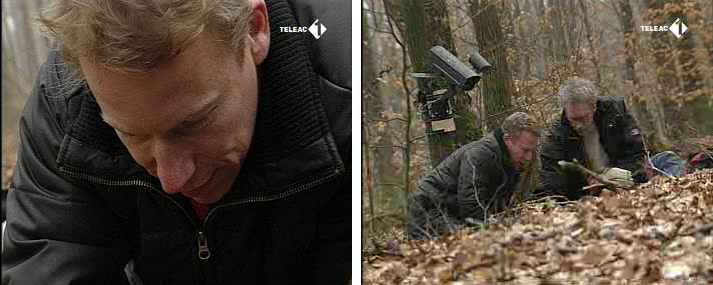
\includegraphics[scale=.7]{images/hard_cut_example.png}
	\caption{These two consecutive frames form a hard cut.}
	\label{fig:hard_cut_example}
\end{figure}

To detect hard cuts, we therefore want to apply a similarity measure to two sequent frames. 
In our case, we represent frames using their color histograms. 
Each frame has 3 color channels (red, green, blue) and therefore 3 histograms.
The difference between two frames is then the difference between the histograms.
The histogram difference can be represented as an \emph{3*n}-dimensional vector, where \emph{n} is the number of bins in a color histogram. 
We then are presented with a binary classification task (cut or not) in a \emph{3*n}-dimensional space. \\
In a next step, the dimensionality can be reduced by simply adding up the vector elements. 
This step is justifiable, since it does not matter which color changed and how much, but the sum of changes in all color channels. 
We will evaluate both approaches later.
To do the actual classification we train an SVM classifier on a labeled training set.
We transform the input space into a higher dimensional feature space by using a kernelized decision function. The commonly used radial basis function (RBF) kernel is employed. 
$$K(x_i,x_j) = exp(-\lambda || x_i - x_j ||^2)$$ 
where $\lambda$ denotes the width of the kernel and $x_i, x_j $ are vectors from the training set. The complexity parameter C for the soft-margin SVM, as well as other parameters are found by using a function, which performs k-fold cross-validation to automatically choose the best parameters.
